% Force paper II to be before paper III in the reference list
%\nocite{Henney:2018a}

\section{Introduction}
\label{sec:intro}


%%
%% Circumstances when bowshocks arise
%%

The archetypal bow shock is formed when a solid body moves
supersonically through a compressible fluid.  Terrestrial examples
include the atmospheric re-entry of a space capsule, or the sonic boom
produced by a supersonic jet \citep{van-Dyke:1982a}.  In astrophysics
the term bow shock is employed more widely, to refer to many different
types of curved shocks that have approximate cylindrical symmetry.
Instead of a solid body, astrophysical examples usually involve the
interaction of \emph{two} supersonic flows, such as the situation of a
stellar wind emitted by a star that moves supersonically through the
interstellar medium \citep{van-Buren:1988a, Kobulnicky:2010a,
  van-Marle:2011a, Mackey:2012b, Mackey:2015a}.  In such cases, two
shocks are generally produced, one in each flow.  Sometimes,
especially in heliospheric studies \citep{Zank:1999a, Scherer:2014a},
the term ``bow shock'' is reserved for the shock in the ambient
medium, with the other being called the ``wind shock'' or
``termination shock''.  However, in other contexts such as colliding
wind binaries \citep{Stevens:1992a, Gayley:2009a} such a distinction
is not so useful.  

%% 
%% Examples of astrophysical bow shocks
%%

\begin{figure}
  \centering
  \bigskip
  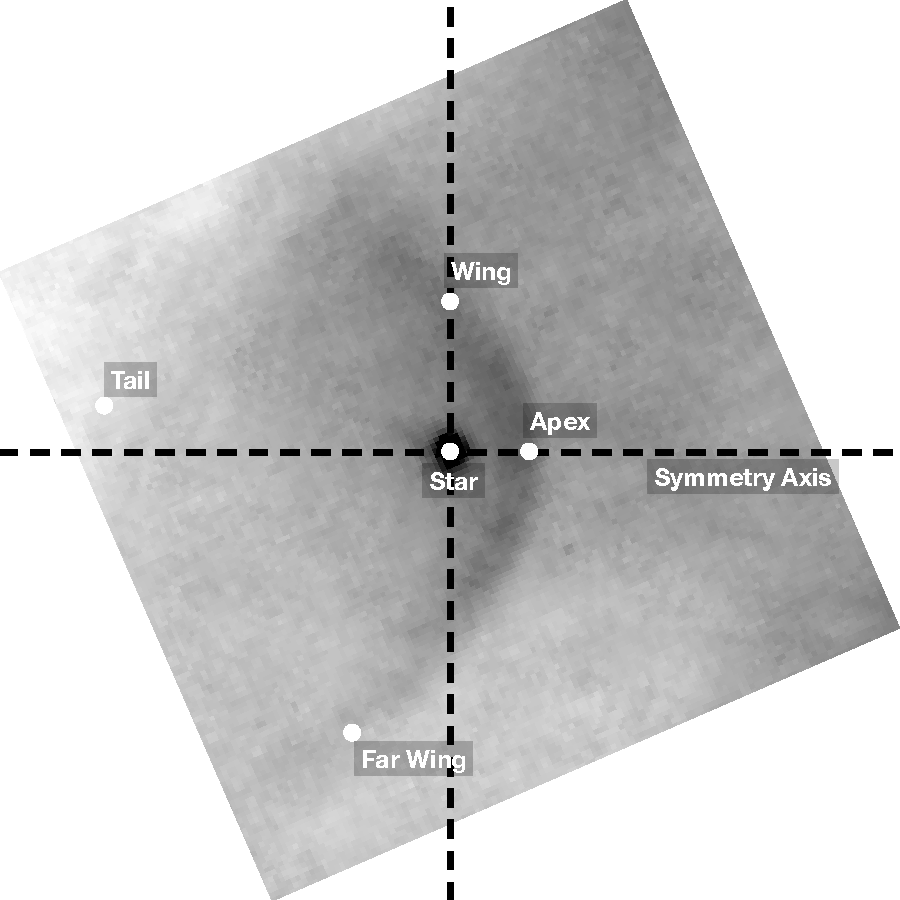
\includegraphics[width=0.9\linewidth]{figs/bow-terminology}
  \caption{Descriptive terminology for a stellar bow shock.  The apex
    is the closest approach of the bow to the star, while the wings
    are the parts of the bow that curve back past the star.}
  \label{fig:bow-terminology}
\end{figure}
A further class of astrophysical bow shock is driven by highly
collimated, supersonic jets of material, such as the Herbig Haro
objects \citep{Schwartz:1978b, Hartigan:1987a} that are powered by
jets from young stars or protostars.  Additional examples are seen in
planetary nebulae \citep{Phillips:2010a, Meaburn:2013a}, active
galaxies \citep{Wilson:1987a}, and in galaxy clusters
\citep{Markevitch:2002a}.  In the jet-driven case, the term ``working
surface'' is often applied to the entire structure comprising the two
shocks plus the shocked gas in between them, separated by a
\textit{contact discontinuity}.  The working surface may be due to the
interaction of the jet with a relatively quiescent medium, or may be an
``internal working surface'' within the jet that is due to
supersonic temporal variations in the flow velocity
\citep{Raga:1990a}.

In empirical studies the relationship between these theoretical
constructs and the observed emission structures is not always clear.
In such cases the term ``bow shock'' is often used in a more general
sense to refer to the entire arc of emission.  In this paper, we will
concentrate on \textit{stellar bow shocks}, in which the position of
the star can serve as a useful reference point for describing the bow
shape.  The empirical terminology that we will employ is illustrated
in Figure~\ref{fig:bow-terminology}.  The \textit{apex} is the point
of closest approach of the bow to the star, which lies on the
approximate symmetry axis, and the region around the apex is sometimes
referred to as the \textit{head} of the bow.  The \textit{wings} are
the swept-back sides of the bow, which lie in a direction from the
star that is orthogonal to the axis, with the \textit{far wings} being
the wing region farthest from the apex. Finally, the \textit{tail} is
the region near the axis but in the opposite direction from the apex.

\begin{figure}
  % 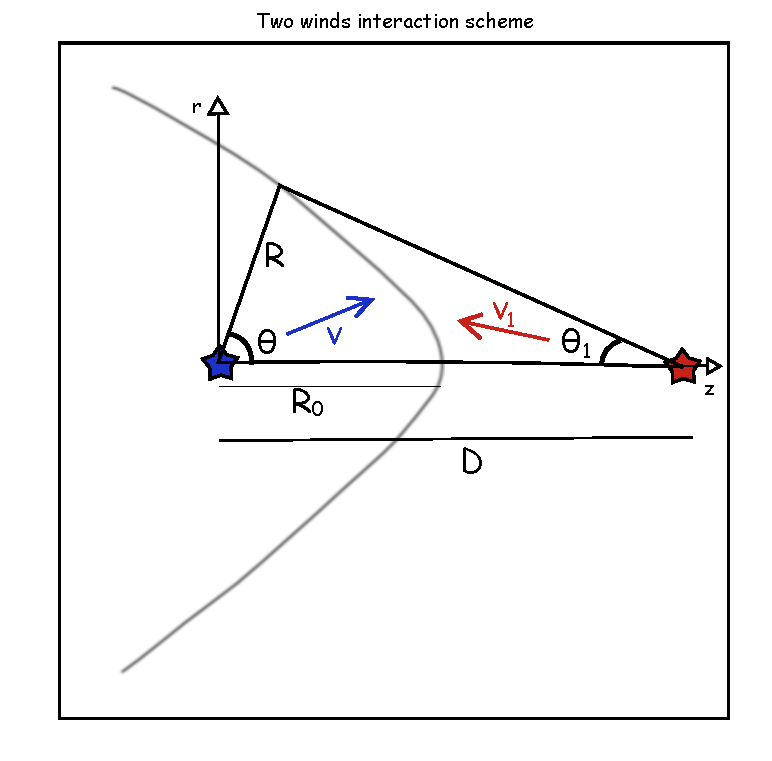
\includegraphics[width=\linewidth]{2winds-scheme}
  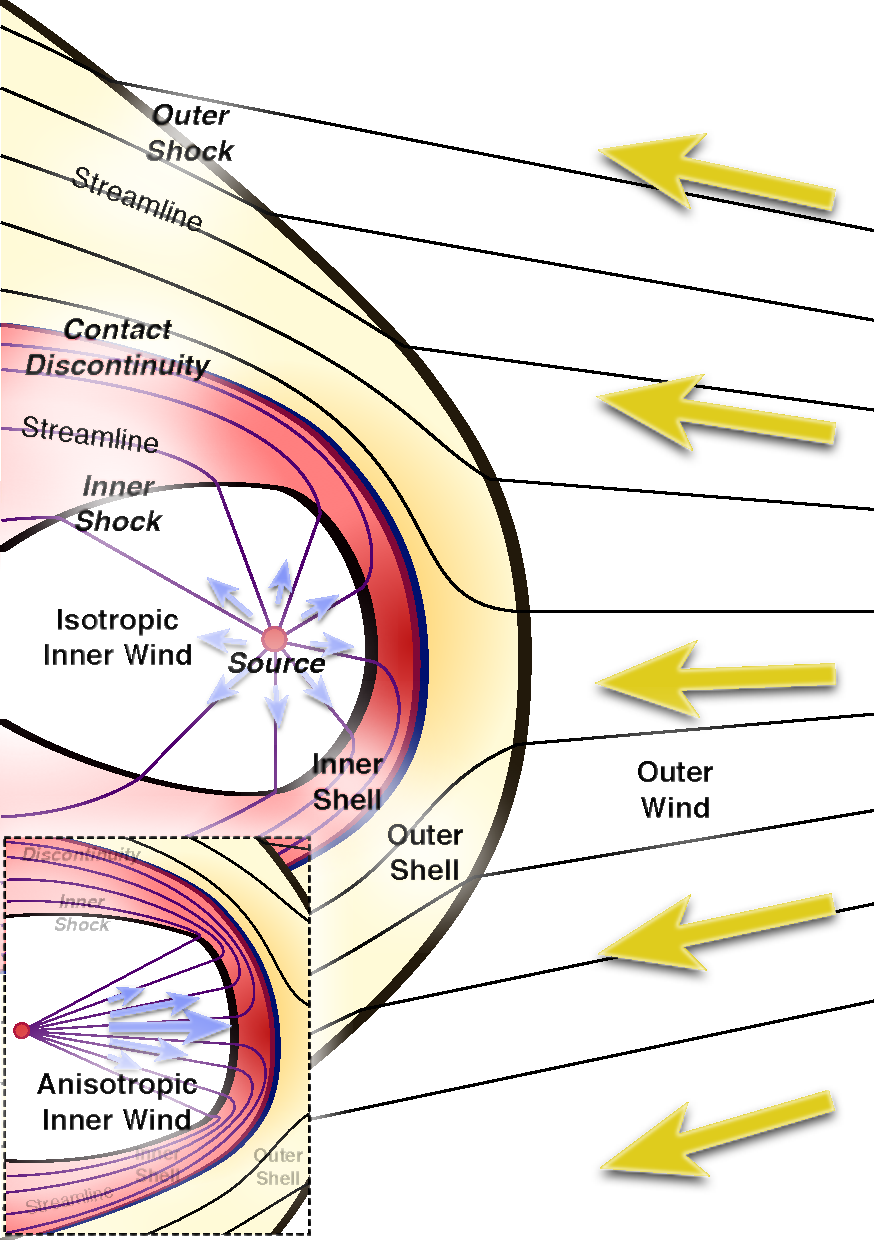
\includegraphics[width=\linewidth]{figs/generic-bowshock}
  \caption{Quasi-stationary bow shock structure formed by the
    interaction of two supersonic winds.  Lower-left inset box shows
    the case where the inner wind is anisotropic. The streamlines
    (thin lines) are drawn to be qualitatively realistic: they are
    straight in regions of hypersonic flow, but curved in subsonic
    regions, responding to pressure gradients in the shocked
    shells. Streamline slopes are discontinuous across oblique
    shocks.}
\label{fig:2-winds}
\end{figure}
\newcommand\Mach{\ensuremath{\mathcal{M}}} Figure~\ref{fig:2-winds}
shows an idealized schematic of how a double bow-shock shell is formed
from the interaction of two supersonic streams: an \textit{inner wind}
and an \textit{outer wind}, with the inner wind being the weaker of
the two (in terms of momentum), so that the shell curves back around
the inner source.  The outer wind may be from another star, or may be
a larger scale flow of the interstellar medium, such as the
\textit{champagne flow} produced by the expansion of an \hii{} region
away from a molecular cloud \citep{Tenorio-Tagle:1979a, Shu:2002a,
  Medina:2014a}.  Alternatively, it may be due to the supersonic
motion of the inner source through a relatively static medium, in
which case the outer wind will not be divergent as shown in the figure
but rather plane-parallel.  The thickness of the shocked shells at the
apex depends on the Mach number, \Mach{}, of the flows and the
efficiency of the post-shock cooling.  For sufficiently strong
cooling, the post-shock cooling zone thickness is negligible and the
shock can be considered isothermal.  In this case, the shell thickness
is of order \(\Mach^{-2}\) times the source-apex separation
\citep{Henney:2002a}, which can become very small for high Mach
numbers.  The shell thickness will tend to increase towards the wings,
due to the increasing shock obliqueness, which reduces the
perpendicular Mach number.

\begin{figure}
  \centering
  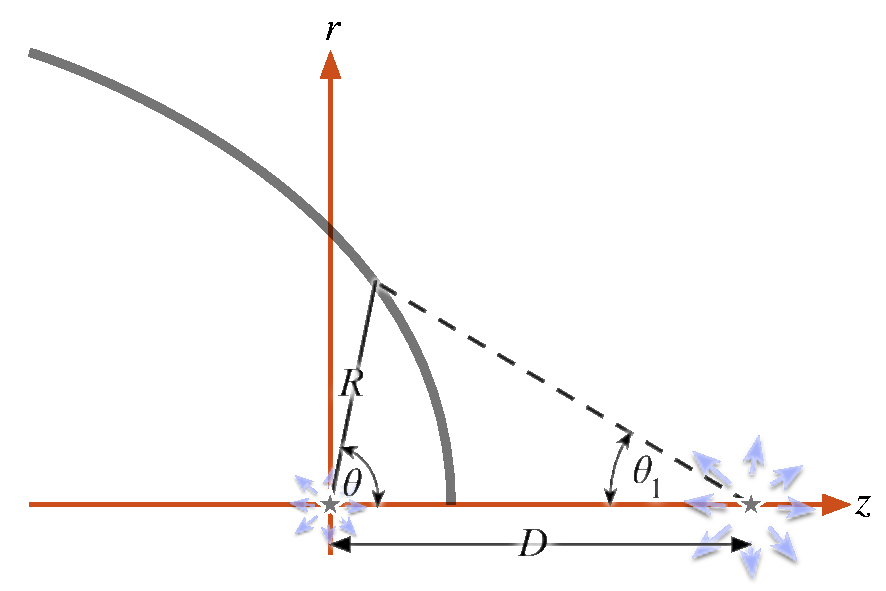
\includegraphics[width=\linewidth]{figs/bowshock-crw-variables}
  \caption[]{Schematic diagram of cylindrically symmetric two-wind
    interaction problem in the thin-shell limit, following
    \citet{Canto:1996}.}
  \label{fig:crw-schema}
\end{figure}
In the extreme thin-shell limit, the entire bow structure can be
treated as a surface.  The bow radius measured from the inner source
(star) is \(R(\theta, \phi)\), where \(\theta\) is the polar angle, measured from
the star-apex axis, and \(\phi\) is the azimuthal angle, measured around
that axis.  Assuming cylindrical symmetry about the axis, this reduces
to \(R(\theta)\), which is illustrated in Figure~\ref{fig:crw-schema},
following \citet{Canto:1996}.  The separation between the two sources
is \(D\) and the complementary angle, as measured at the position of
the outer source, is \(\theta_1\).  The minimum value of \(R(\theta)\) is the
stagnation radius, \(R_0\), which occurs at the apex (\(\theta = 0\)).  In
a steady state, ram-pressure balance on the axis implies that
\begin{equation}
  \label{eq:stagnation-radius}
  \frac{R_0} {D} = \frac{\beta^{1/2}} {1 + \beta^{1/2}} ,
\end{equation}
where \(\beta\) is the momentum ratio between the two winds.  If the winds
are isotropic, with inner wind mass-loss rate \(\dot{M}_{\w}\) and
terminal velocity \(V_{\w}\), while the outer wind has corresponding
values \(\dot{M}_{\w1}\) and \(V_{\w1}\), then the momentum ratio is
\begin{equation}
  \label{eq:beta-definition}
  \beta = \frac{\dot{M}_{\w} V_{\w}} {\dot{M}_{\w1} V_{\w1}} .
\end{equation}
The case where the outer wind is a parallel stream
\citep{Wilkin:1996a} corresponds to the limit \(\beta \to 0\), in which case
\(D\) is no longer a meaningful parameter.

% \TODO{Bow shocks from pulsars and neutron stars
%   \citep{Cordes:1993a, Brownsberger:2014a}.}


The paper is organized as follows.
%
In \S~\ref{sec:plan-alat-bow} we outline the geometric parameters that
are necessary for describing bow shapes and introduce two
dimensionless ratios: planitude and alatude.
%
In \S~\ref{sec:projection} we derive general results for the
projection of bow shapes on to the plane of the sky.
%
In \S~\ref{sec:conic} we apply the results to the simplest possible
class of geometric bow models: the quadrics of revolution, which
comprise spheroids, paraboloids, and hyperboloids, each of which
occupies a distinct region of the planitude--alatude plane.
%
In \S~\ref{sec:crw-scenario} we consider thin-shell hydrodynamic
models for the parallel-stream case (wilkinoids) and wind-wind case
(cantoids), including extension to an anisotropic inner wind
(ancantoids).  We calculate the location of the models in the
planitude--alatude plane as a function of the inclination of the bow
shock axis to the plane of the sky.
%
In \S~\ref{sec:more-realistic-bow} we test our methods against the
results of more realistic numerical simulations of bow shocks,
including the derivation of the shape parameters from maps of infrared
dust emission.
%
In \S~\ref{sec:conc} we summarise our results and outline how
following papers will apply these ideas to observations and to a more
extensive set of models and numerical simulations.


% The bow shocks we consider are originated by a source located at the
% origin, emitting a wind with a mass loss rate of $\dot{M}_{\w}$ and a
% terminal (supersonic) velocity $v_{\w}$. This wind interacts with another
% wind originated by another source located at a distance $D$ from the
% first one.  The mass loss rate of the second source is $\dot{M}_{\w1}$
% and the terminal velocity is $v_{\w1}$. The momentum of the wind of the
% second source is higher than the momentum of the first one, and the
% resultant bow shock is stationary due to pressure balance.

\section{Planitude and alatude of bow shapes}
\label{sec:plan-alat-bow}

\begin{figure}
  \centering
  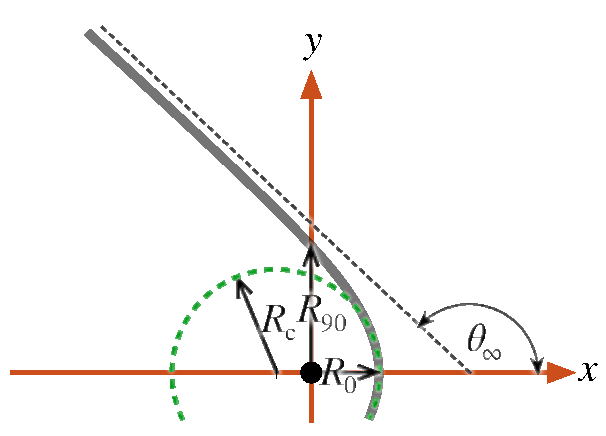
\includegraphics[width=\linewidth]{figs/characteristic-radii}
  \caption[]{Parameters for characterizing a bow shape.  Bow radius
    from the star, measured parallel (\(R_0\)) and perpendicular
    (\(R_{90}\)) to the symmetry axis, together with radius of
    curvature (\(R_{\C}\)) at apex and asymptotic opening angle
    (\(\theta_\infty\)) of the far wings. }
  \label{fig:characteristic-radii}
\end{figure}

The stagnation radius \(R_0\) describes the linear scale of the bow
shock, but in order to characterize its shape more parameters are
required.  To efficiently capture the diversity of bow shapes, we
propose the parameters shown in Figure~\ref{fig:characteristic-radii}.
The perpendicular radius \(R_{90}\) is the value of \(R(\theta)\) at
\(\theta = 90^\circ\), whereas \(R_{\C}\) is the radius of curvature of the bow at
the apex (\(\theta = 0\)), which in cylindrical symmetry simplifies to
\begin{equation}
  \label{eq:radius-curvature}
  R_{\C} 
  % = R_0 \Biggl[ 1
  % - \frac{1} {R_0} \left.\frac{d^2\! R} {d\,\theta^2}\right|_{\theta = 0} \Biggr]^{-1}
  = \frac{R_0^2}{R_0 - R_{\theta\theta,0}} \ , 
\end{equation}
where \(R_{\theta\theta,0}\) is \(d^2 \!R / d\theta^2\) evaluated at \(\theta = 0\).

A fourth parameter is the asymptotic opening angle of the far wings,
\(\theta_\infty\), which is useful in the case that the wings are asymptotically
conical.  However, in many bow shocks the wings tend towards the
asymptotic angle only slowly, making \(\theta_\infty\) difficult to measure,
especially since the emission from the far wings is often weak at
best.  In contrast, the three radii, \(R_0\), \(R_{90}\), and
\(R_{\C}\). are straightforward to determine from observations.  One
simple method to estimate the radius of curvature is to make use of
the Taylor expansion\footnote{%
  This method assumes both that \(R(\theta)\) is even (true for a
  cylindrically symmetric bow) and that the orientation of the axis is
  already known.  Generalization to cases where these assumptions do
  not hold is discussed in \citet{Henney:2018b}.} %
of \(R(\theta)\) about the apex (with \(\theta\) in
radians):
\begin{equation}
  \label{eq:taylor-R-theta}
  R(\theta) = R_0 + \frac12 R_{\theta\theta,0} \,\theta^2 + \mathcal{O}(\theta^4) \ ,
\end{equation}
so that fitting a polynomial in \(\theta^2\) to \(R(\theta)\) for
\(|\theta| < \Delta\theta \) yields \(R_0\) and \(R_{\theta\theta,0}\) from the first two
coefficients, and hence \(R_{\C}\) from
equation~\eqref{eq:radius-curvature}.  Experience has shown that
\(\Delta\theta = 30^\circ\) and three terms in the polynomial are good choices,
where the third term is used only as a monitor (if the co-efficient of
\(\theta^4\) is not small compared with \(R_0\), then it may indicate a
problem with the fit).

Since we have three radii, we can construct two independent
dimensionless parameters:
\begin{align}
  \label{eq:planitude}
  \text{Planitude} \quad \Pi & \equiv  \frac{R_{\C}} {R_0} \\
  \label{eq:alatude}
  \text{Alatude} \quad \Lambda & \equiv  \frac{R_{90}} {R_0}
\end{align}
and these will be the principal shape parameters that we will use in
the remainder of the paper.  The \textit{planitude}, \(\Pi\), is a
measure of the flatness of the head of the bow around the apex, while
the \textit{alatude}, \(\Lambda\), is a measure of the openness of the bow
wings.  Although ``planitude'' can be found in English dictionaries,
``alatude'' is a new word that we introduce here, derived from the
latin \textit{ala} for ``wing''.

Several previous studies have discussed the relation between
\(R_{90}\) and \(R_0\) as a diagnostic of bow shape (for example
\citealp{Robberto:2005, Cox:2012a, Meyer:2016a}), but as far as we
know, we are the first to include \(R_{\C}\).  \citet{Robberto:2005}
\S~4.2 use the ratios \(R_0/D\) and \(R_{90}/D\) in analyzing proplyd
bow shapes in the Trapezium cluster in the center of the Orion Nebula
\citep{Hayward:1994a, Garcia-Arredondo:2001a, Smith:2005a}.  In that
case, the source of the outer wind is known, and so \(D\) is
well-determined (at least, in projection), but for many bow shocks
\(D\) is not known, and is not even defined for the moving-star or
parallel-stream case. \citet{Cox:2012a} \S~4.1 compare the observed
shapes of bow shocks around cool giant stars with an analytic model,
and use \(A\) and \(B\) for the projected values of \(R_0\) and
\(R_{90}\), respectively (see next section for discussion of
projection effects).  \citet{Meyer:2016a} \S~3.2 analyze the
distribution of \(R_0 / R_{90}\) (the reciprocal of our \(\Lambda\)) for
hydrodynamic simulations of bow shocks around runaway OB stars.

% In order to contrast different bow shock models, we derive a set of
% measurable radii. Each model used should predict them and these
% predictions can be compared with observations.
% \begin{itemize}
% \item Radius at axis of symmetry. Denoted as $R_0$.
% \item Radius of Curvature at the axis of symmetry. Denoted as $R_{\C}$
% \item Radius at the perpendicular direction to the symmetry
%   axis. Denoted as $R_{90}$
% \item For open bow shocks, the asymptotic angle. Denoted as
%   $\theta_\infty$
% \end{itemize}



%% 
%% Restriction to cylindrical symmetry
%% 

% For simplicity, the current paper is restricted to cylindrically
% symmetric bow shock shapes. 

%%
%% Effects of instabilities
%%


%%% Local Variables:
%%% mode: latex
%%% TeX-master: "quadrics-bowshock"
%%% End:
